\documentclass[xcolor=table]{beamer}
\mode<presentation>
{
  \usetheme{Warsaw}
  \definecolor{mcgarnet}{rgb}{0.38, 0, 0.08}
  \definecolor{mcgray}{rgb}{0.6, 0.6, 0.6}
  \setbeamercolor{structure}{fg=mcgarnet,bg=mcgray}
  %\setbeamercovered{transparent}
}


\usepackage{xcolor}
\usepackage[english]{babel}
\usepackage[latin1]{inputenc}
\usepackage{times}
\usepackage[T1]{fontenc}
\usepackage{tikz}
\usepackage{graphicx}
\usepackage{fancyvrb}
\usepackage{adjustbox}

\newcommand{\imagesource}[1]{{\centering\hfill\break\hbox{\scriptsize Image Source:\thinspace{\small\itshape #1}}\par}}

\title{07 - Loops and Formatting}


\author{Dr. Robert Lowe\\}

\institute[Maryville College] % (optional, but mostly needed)
{
  Division of Mathematics and Computer Science\\
  Maryville College
}

\date[]{}
\subject{}

\pgfdeclareimage[height=0.5cm]{university-logo}{images/Maryville-College}
\logo{\pgfuseimage{university-logo}}


\AtBeginSection[]
{
  \begin{frame}<beamer>{Outline}
    \tableofcontents[currentsection]
  \end{frame}
}


\begin{document}

\begin{frame}
  \titlepage
\end{frame}

\begin{frame}{Outline}
  \tableofcontents
\end{frame}


% Structuring a talk is a difficult task and the following structure
% may not be suitable. Here are some rules that apply for this
% solution: 

% - Exactly two or three sections (other than the summary).
% - At *most* three subsections per section.
% - Talk about 30s to 2min per frame. So there should be between about
%   15 and 30 frames, all told.

% - A conference audience is likely to know very little of what you
%   are going to talk about. So *simplify*!
% - In a 20min talk, getting the main ideas across is hard
%   enough. Leave out details, even if it means being less precise than
%   you think necessary.
% - If you omit details that are vital to the proof/implementation,
%   just say so once. Everybody will be happy with that.

\section{Repeating Code}

\begin{frame}{Loop Overview}
  \begin{itemize}[<+->]
    \item Loops allow segments of code to be repeated.
    \item Loop operation is similar to branches; they are based on true/false conditions.
    \item C++ provides 3 types of loops: \texttt{while}, \texttt{do..while}, and \texttt{for}.
  \end{itemize}
\end{frame}

\begin{frame}[fragile]{The While Loop}
  \begin{columns}
    \column{0.5\textwidth}

    \begin{block}{While Loop Syntax}
      \verb!while(! \textit{condition} \verb!)! 
      \newline\verb!    ! \textit{statement/block}
    \end{block}
    
    \vspace{0.5cm}

    \begin{itemize}[<+(1)->]
      \item If the \textit{condition} is true, the loop body is executed.
      \item After the loop body executes, the process begins again.
      \item How many times will the loop body execute?
      \begin{itemize}
          \item Zero or more times!
      \end{itemize}
    \end{itemize}

    \column{0.5\textwidth}
    \begin{center}
      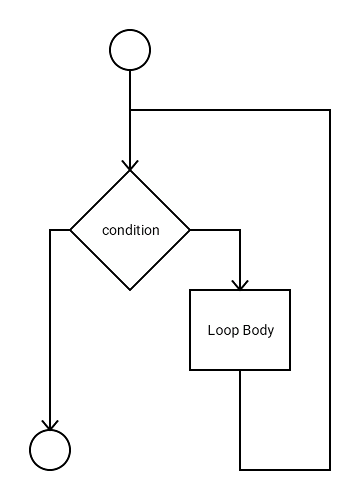
\includegraphics[width=0.8\textwidth]{images/while}
    \end{center}
  \end{columns}
\end{frame}

\begin{frame}[fragile]{Example: \texttt{count.cpp}}
  \begin{itemize}[<+(1)->]
      \item \texttt{count.cpp} is in your \texttt{examples/07-Loops} directory.
      \item Examine this file (use \texttt{less})
      \item Compile and run the count program.
      \item The loop part of the file is shown below:
  \end{itemize}

  \begin{BVerbatim}
    //start at zero
    num = 0;

    //count to 10
    while(num <= 10) {
        //display the number
        cout << num << endl;

        //go to the next number
        num = num + 1;
    }
  \end{BVerbatim}
\end{frame}

\begin{frame}[fragile]{Increment and Decrement Operators}
  \begin{itemize}[<+->]
    \item Adding (or subtracting) 1 to a variable is quite common in loops.
    \item To facilitate this, C++ has an increment operator (\verb#++#) and a decrement operator(\verb#--#).
    \item Both operators have a prefix version:
      \newline\verb#++x#
      \newline\verb#--x#
    \item Both operators have a postfix version:
      \newline\verb#x++#
      \newline\verb#x--#
  \end{itemize}
\end{frame}

\begin{frame}[fragile]{Prefix Increment and Decrement}
  \begin{block}{Prefix Increment and Decrement}
    The prefix operators increment the variable and returns the \textbf{new} value.
  \end{block}

  \uncover<+->{\textbf{Sample Evaluation}}
  \rowcolors{2}{gray!25}{white}
  \begin{tabular}{|l|c|r|}
    \hline
    \rowcolor{white}
    \textbf{Statement} & \textbf{Screen Output} & \textbf{Value of X}\\
    \hline
    \uncover<+->{\texttt{x=0;} & \texttt{} & Undefined} \\
    \uncover<+->{\texttt{0;} & \texttt{} & 0}\\
    \uncover<+->{\texttt{cout << ++x;} & \texttt{} & 0}\\
    \uncover<+->{\texttt{cout << 1;} & \texttt{} & 1}\\
    \uncover<+->{\texttt{cout;} & \texttt{1} & 1}\\
    \hline
  \end{tabular}
\end{frame}

\begin{frame}{Postfix Increment and Decrement}
  \begin{block}{Postfix Increment and Decrement}
    The postfix operators increment the variable and returns the \textbf{old} value.
  \end{block}

  \uncover<+->{\textbf{Sample Evaluation}}
  \rowcolors{2}{gray!25}{white}
  \begin{tabular}{|l|c|r|}
    \hline
    \rowcolor{white}
    \textbf{Statement} & \textbf{Screen Output} & \textbf{Value of X}\\
    \hline
    \uncover<+->{\texttt{x=0;} & \texttt{} & Undefined}\\
    \uncover<+->{\texttt{0;} & \texttt{} & 0}\\
    \uncover<+->{\texttt{cout << x++;} & \texttt{} & 0}\\
    \uncover<+->{\texttt{cout << 0;} & \texttt{} & 1}\\
    \uncover<+->{\texttt{cout;} & \texttt{0} & 1}\\
    \hline
  \end{tabular}
\end{frame}

\begin{frame}[fragile]{Operator Precedence (thus far)}
  \begin{adjustbox}{max totalheight=0.8\textheight}
    \begin{tabular}{|l|l|l|}
        \hline
        \textbf{Operator} & \textbf{Description} & \textbf{Associativity} \\
        \hline
        \texttt{a++}, \verb#a--# & Postfix increment and decrement & Left-to-Right\\
        \hline
        \texttt{not}, \texttt{!} & Logical Not & Right-to-Left\\
        \texttt{++a}, \verb#--a# & Prefix increment and decrement &  \\
        \hline
        \texttt{a*b}, \texttt{a/b}, \texttt{a\%b} & Multiply, Divide, Modulus & Left-to-Right\\
        \hline
        \texttt{a+b}, \texttt{a-b} & Addition and Subtraction & Left-to-Right\\
        \hline
        \texttt{<<} , \texttt{>>} & Insertion and Extraction & Left-to-Right \\
        \hline
        \texttt{<}, \texttt{<=} & Relational Operators & Left-to-Right\\
        \texttt{>}, \texttt{>=} & & \\
        \hline
        \texttt{==}, \texttt{!=} & Equality Operators & Left-to-Right\\
        \hline
        \texttt{and}, \texttt{\&\&} & Logical And & Left-to-Right\\
        \hline
        \texttt{or}, \texttt{||} & Logical Or & Left-to-Right\\
        \hline
        \texttt{=},  & Assignment and Assignment & Right-to-Left \\
        \texttt{+=}, \texttt{-=} & & \\
        \texttt{*=}, \texttt{/=} & & \\
        \texttt{\%=} & & \\
        \hline
    \end{tabular}
  \end{adjustbox}
\end{frame}

\begin{frame}{Lab Activity: Using Increment Operator With \texttt{count.cpp}}
  \begin{enumerate}[<+->]
    \item Copy \texttt{count.cpp} to your \texttt{labs/week4} directory.
    \item Open your copy in your favorite text editor, and locate the following line:
      \newline\texttt{num = num + 1;}
    \item Change this line to:
      \newline\texttt{num++;}
    \item Test your program to make sure it still works.
    \item \textbf{Discuss}: Does it matter if we use the prefix or postfix operator in this case?
  \end{enumerate}
\end{frame}

\begin{frame}[fragile]{Lab Activity: \texttt{count2.cpp}}

  \uncover<+->{We are going to create a new program that counts from \texttt{start} to \texttt{end} by some \texttt{increment}}.
  \newline\uncover<+->{For example, count from 0 to 100 by fives}
  \begin{enumerate}[<+->]
    \item Copy \texttt{count.cpp} to \texttt{count2.cpp}
    \item Open \texttt{count2.cpp} in the text editor of your choice.
    \item Add variables for \texttt{start}, \texttt{end}, and \texttt{increment}.
    \begin{BVerbatim}

    int start; //The first number
    int end;   //The last number
    int increment;  //The amount to add each time
    \end{BVerbatim}
    \item Modify the program so that the first thing it does is prompt the user and read in these three variables.

  \end{enumerate}
\end{frame}


\begin{frame}[fragile]{Lab Activity: \texttt{count2.cpp} Continued}
  \begin{enumerate}[<+->][4]
    \item Modify the program so that instead of starting at zero, it starts at \texttt{start}.\newline
    \begin{BVerbatim}

    //start at start
    num = start;
    \end{BVerbatim}

    \item Modify the program so that instead of adding 1 to \texttt{num} each time through the loop, it adds \texttt{increment}.\newline
    \begin{BVerbatim}

        //go to the next number
        num += increment;
    \end{BVerbatim}

    \item Compile and test your program.
  \end{enumerate}
\end{frame}

\begin{frame}{Loop Problem: Fahrenheit Scale}
  \begin{columns}
    \column{0.7\textwidth}
    \begin{itemize}[<+->]
      \item In 1724, Daniel Fahrenheit proposed a precise way to measure temperature.
      \item His scale was reproducible and brilliant!
      \item 0 was fixed at the temperature achieved by mixing equal quantities of water, ice, and ammonia chloride.
      \item 100 is the temperature of healthy blood.
      \item The scale is divided into equal marks from 0 to 100.
    \end{itemize}

    \column{0.3\textwidth}
    \begin{center}
      
\includegraphics[width=0.9\textwidth]{images/fahrenheit}
      {\tiny\newline\textbf{Daniel Fahrenheit} \newline Image Source: \url{https://en.wikipedia.org/wiki/Daniel_Gabriel_Fahrenheit}}
    \end{center}
  \end{columns}
\end{frame}

\begin{frame}{Loop Problem: Celsius Scale}
  \begin{columns}
    \column{0.7\textwidth}
    \begin{itemize}[<+->]
      \item In 1742, Anders Celsius proposed a new scale.
      \item Celsius's scale was, I think you'll agree, completely unrelatable.
      \item For 0, Celsius used the freezing point of water at sea level.
      \item For 100, Celsius used the boiling point of water at sea level.
      \item Only the United States holds fast to the bitter salt slush to blood scale.
      \item God bless the USA, and long live the imperial system of units!
    \end{itemize}

    \column{0.3\textwidth}
    \begin{center}
      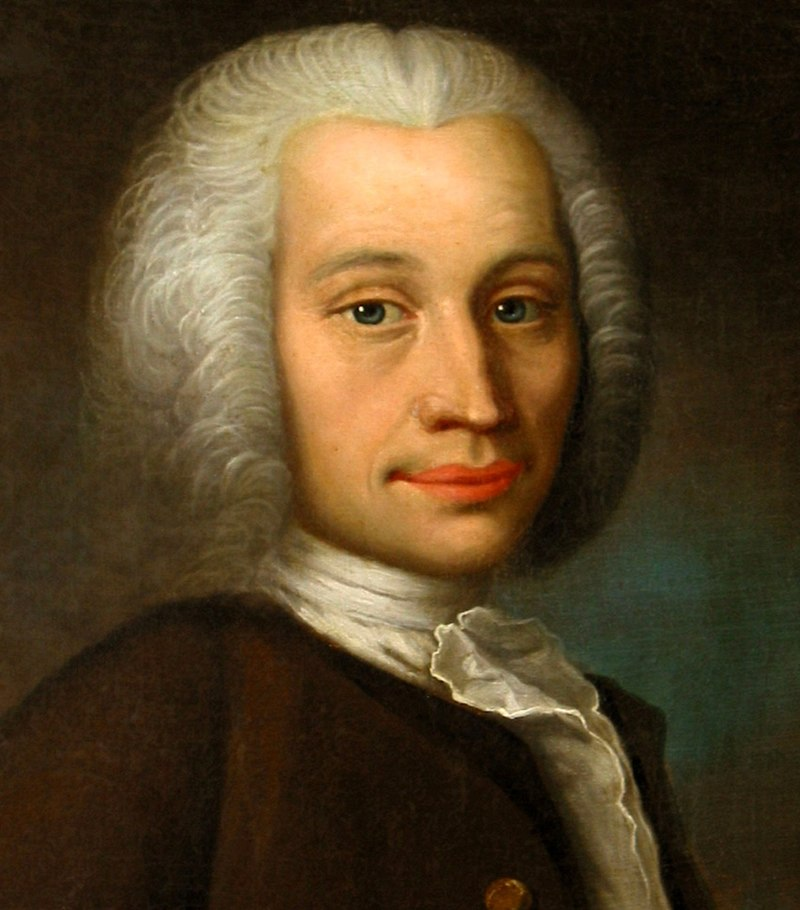
\includegraphics[width=0.9\textwidth]{images/celsius}
      {\tiny\newline\textbf{Anders Celsius}\newline Image Source: \url{https://en.wikipedia.org/wiki/Anders_Celsius}}
    \end{center}
  \end{columns}
\end{frame}

\begin{frame}{Loop Problem: Fahrenheit to Celsius Table}
  \begin{itemize}[<+->]
    \item In reluctant deference to the people who use the inferior scale (96\% of the world's population), we will produce a table converting from Fahrenheit to Celsius.
    \item The table will allow the user to specify the starting temperature, ending temperature, and increment.
    \item The table should be nicely formatted.
    \item The formula for doing the conversion is:
    \[
      c = \displaystyle\frac{5}{9} (f - 32)
    \]
    \item Let's talk about the design of this program for a minute.
  \end{itemize}
\end{frame}

\begin{frame}[fragile]{Loop Problem: Fahrenheit to Celsius Table (continued)}
  \begin{enumerate}[<+->]
    \item Copy \texttt{count2.cpp} to \texttt{fahrenheit.cpp}
    \item Change all mentions of the variable \texttt{num} to \texttt{f}
    \item Change all variable types to \texttt{double}
    \item Add a variable \texttt{c}
    \item Alter the program so that the first thing it does is display a welcome message.
      \newline\texttt{Fahrenheit to Celsius Temperature Table}
    \item Just before the \texttt{while} loop,have the program print a header on a line by itself:
      \newline\verb#Fahrenheit  Celsius#
    \item At the beginning of the loop body, add code to compute the Celsius value \texttt{c} from the fahrenheit value \texttt{f}.
    \item Alter the line that prints out \texttt{f} so that it prints the fahrenheit and Celsius temperatures.
    \item Compile and test your program.
  \end{enumerate}
\end{frame}


\section{Formatting}

\begin{frame}{\texttt{cout} and Fields}
  \begin{itemize}[<+->]
      \item \texttt{cout} does its work by translating its input into a string of characters.
      \item Every \texttt{<<} operations that results in output is called a \textbf{field}.
      \item There exist a series of flags which affect how \texttt{cout} performs formats its output.
      \item Managing these flags individually is tedious and painful!
  \end{itemize}
\end{frame}

\begin{frame}{\texttt{iomanip}}
  \begin{itemize}[<+->]
    \item \texttt{iomanip} is a collection of \textbf{input manipulators} that make working with cout easier.
    \item To use \texttt{iomanip} you have to include it:
      \newline\texttt{\#include <iomanip>}
    \item Go ahead and add this to \texttt{fahrenheit.cpp}
  \end{itemize}
\end{frame}

\begin{frame}[fragile]{Setting the Field Width}
  \begin{itemize}[<+->]
    \item Most io manipulators are used inline with insertion operators.
    \item One very handy manipulator is \texttt{setw}, which sets the width of the next filed.
    \item For example, modify the fahrenheit program's line which displays the temperatures:
    \begin{BVerbatim}
        //display the values
        cout << setw(10) << f << "  " 
             << setw(7) << c << endl;
    \end{BVerbatim}
    \item Test and run your programs.  See if you can guess why I selected the numbers 10 and 7.
  \end{itemize}
\end{frame}

\begin{frame}[fragile]{Number Formatting}
  \begin{itemize}[<+->]
      \item The precision of floating point number displays is controlled using the \texttt{set\_precision} function.
      \item In default or normal mode, precision indicates the maximum total number of digits displayed.
      \item In \texttt{fixed} mode, precision indicates the number of digits to the right of the decimal point.
      \item Once set, the numeric mode remains in effect until it is changed.
      \item Just before your loop in \texttt{fahrenheit.cpp} add the following:
      \begin{BVerbatim}
    //set up number format
    cout << fixed << setprecision(2);
      \end{BVerbatim}
      \item Compile and test your program.  Isn't that nice?
  \end{itemize}
\end{frame}

\begin{frame}{Week 4 Lab Requirements}
  For full credit, your week 4 lab directory should contain:
  \begin{enumerate}
    \item A fully corrected \texttt{proportions.cpp}
    \item \texttt{stock.cpp} with working menu messages.
    \item \texttt{count.cpp} using the increment operator.
    \item \texttt{count2.cpp}
    \item \texttt{fahrenheit.cpp} 
  \end{enumerate}
\end{frame}

\end{document}


